\subsection*{Цель работы}

Изучить принцип работы промышленного робота (ПР), приобрести навыки составления программы и методики обучения робота, проверить работу робота в автоматическом режиме.

\subsection*{Устройство программного управления АПС-1}

Устройство АПС-1 предназначено для управления гаммой промышленных роботов типа ``Универсал'', в том числе для управления роботом ``Универсал 5.02''.

В соответствии с принятой классификацией устройств программного управления промышленных роботов, устройство АПС-1 относится к автономным позиционным устройствам. Оно обеспечивает выполнение следующих характерных алгоритмов управления:

\begin{itemize}
    \item формирование управляющей программы путем обучения робота по первому технологическому циклу;
    \item автоматическое независимое и одновременное перемещение подвижных органов маниулятора в заданную точку позиционирования;
    \item ввод-вывод дискретных команд управления электроавтоматикой манипулятора и обслуживаемого оборудования с контролем выполнения каждой команды;
    \item циклическую или пошаговую отработку кадров управляющей программы с программированием времени задержки между кадрами;
    \item последовательную отработку информации, записанной в кадлре, перемещение подвижных органов манипулятора; ввод-вывод команд на манипулятор; вво-вывод команд на обслуживаемое оборудование;
    \item связь с ЭВМ высшего уровня, работающей в режиме диспетчера программы.
\end{itemize}

Промышленный робот ``Универсал 5.02'' предназначен для комплексной механизации и автоматизации технологических процессов в условиях многофункционального производства (массового, крупносерийного и серийного).

Система координат ПР --- полярная.

Степень подвижности - 6.

Степень свободы - 6 (4 транспортные, 2 ориентирующие).

\subsection*{Схема аналогового позиционирования (АПС) манипулятора}

Аналого-позиционная система программного управления АПС-1 предназначена для управления манипуляторами типа ``Универсал'' и модульной конструкцией РПМ-25 в составе роботизированного технологического участка.

АПС состоит из: устройства ввода программы; блока задатчиков; панели настройки; блока индикации; панели управления; платы функционального преобразователя; платы дешифраторов координат 1, 2, 3; платы дешифраторов технологических команд; платы дешифраторов координат 4, 5, 6; платы дешифраторов выдержки времени; платы преобразователя; платы управления циклом; платы реле 1 -- 6; источников питания; пульта обучения.

Рассмотрим функциональную схему аналого-позиционной системы (рисунок~\ref{fig:functional}).

\begin{figure}[ht]
    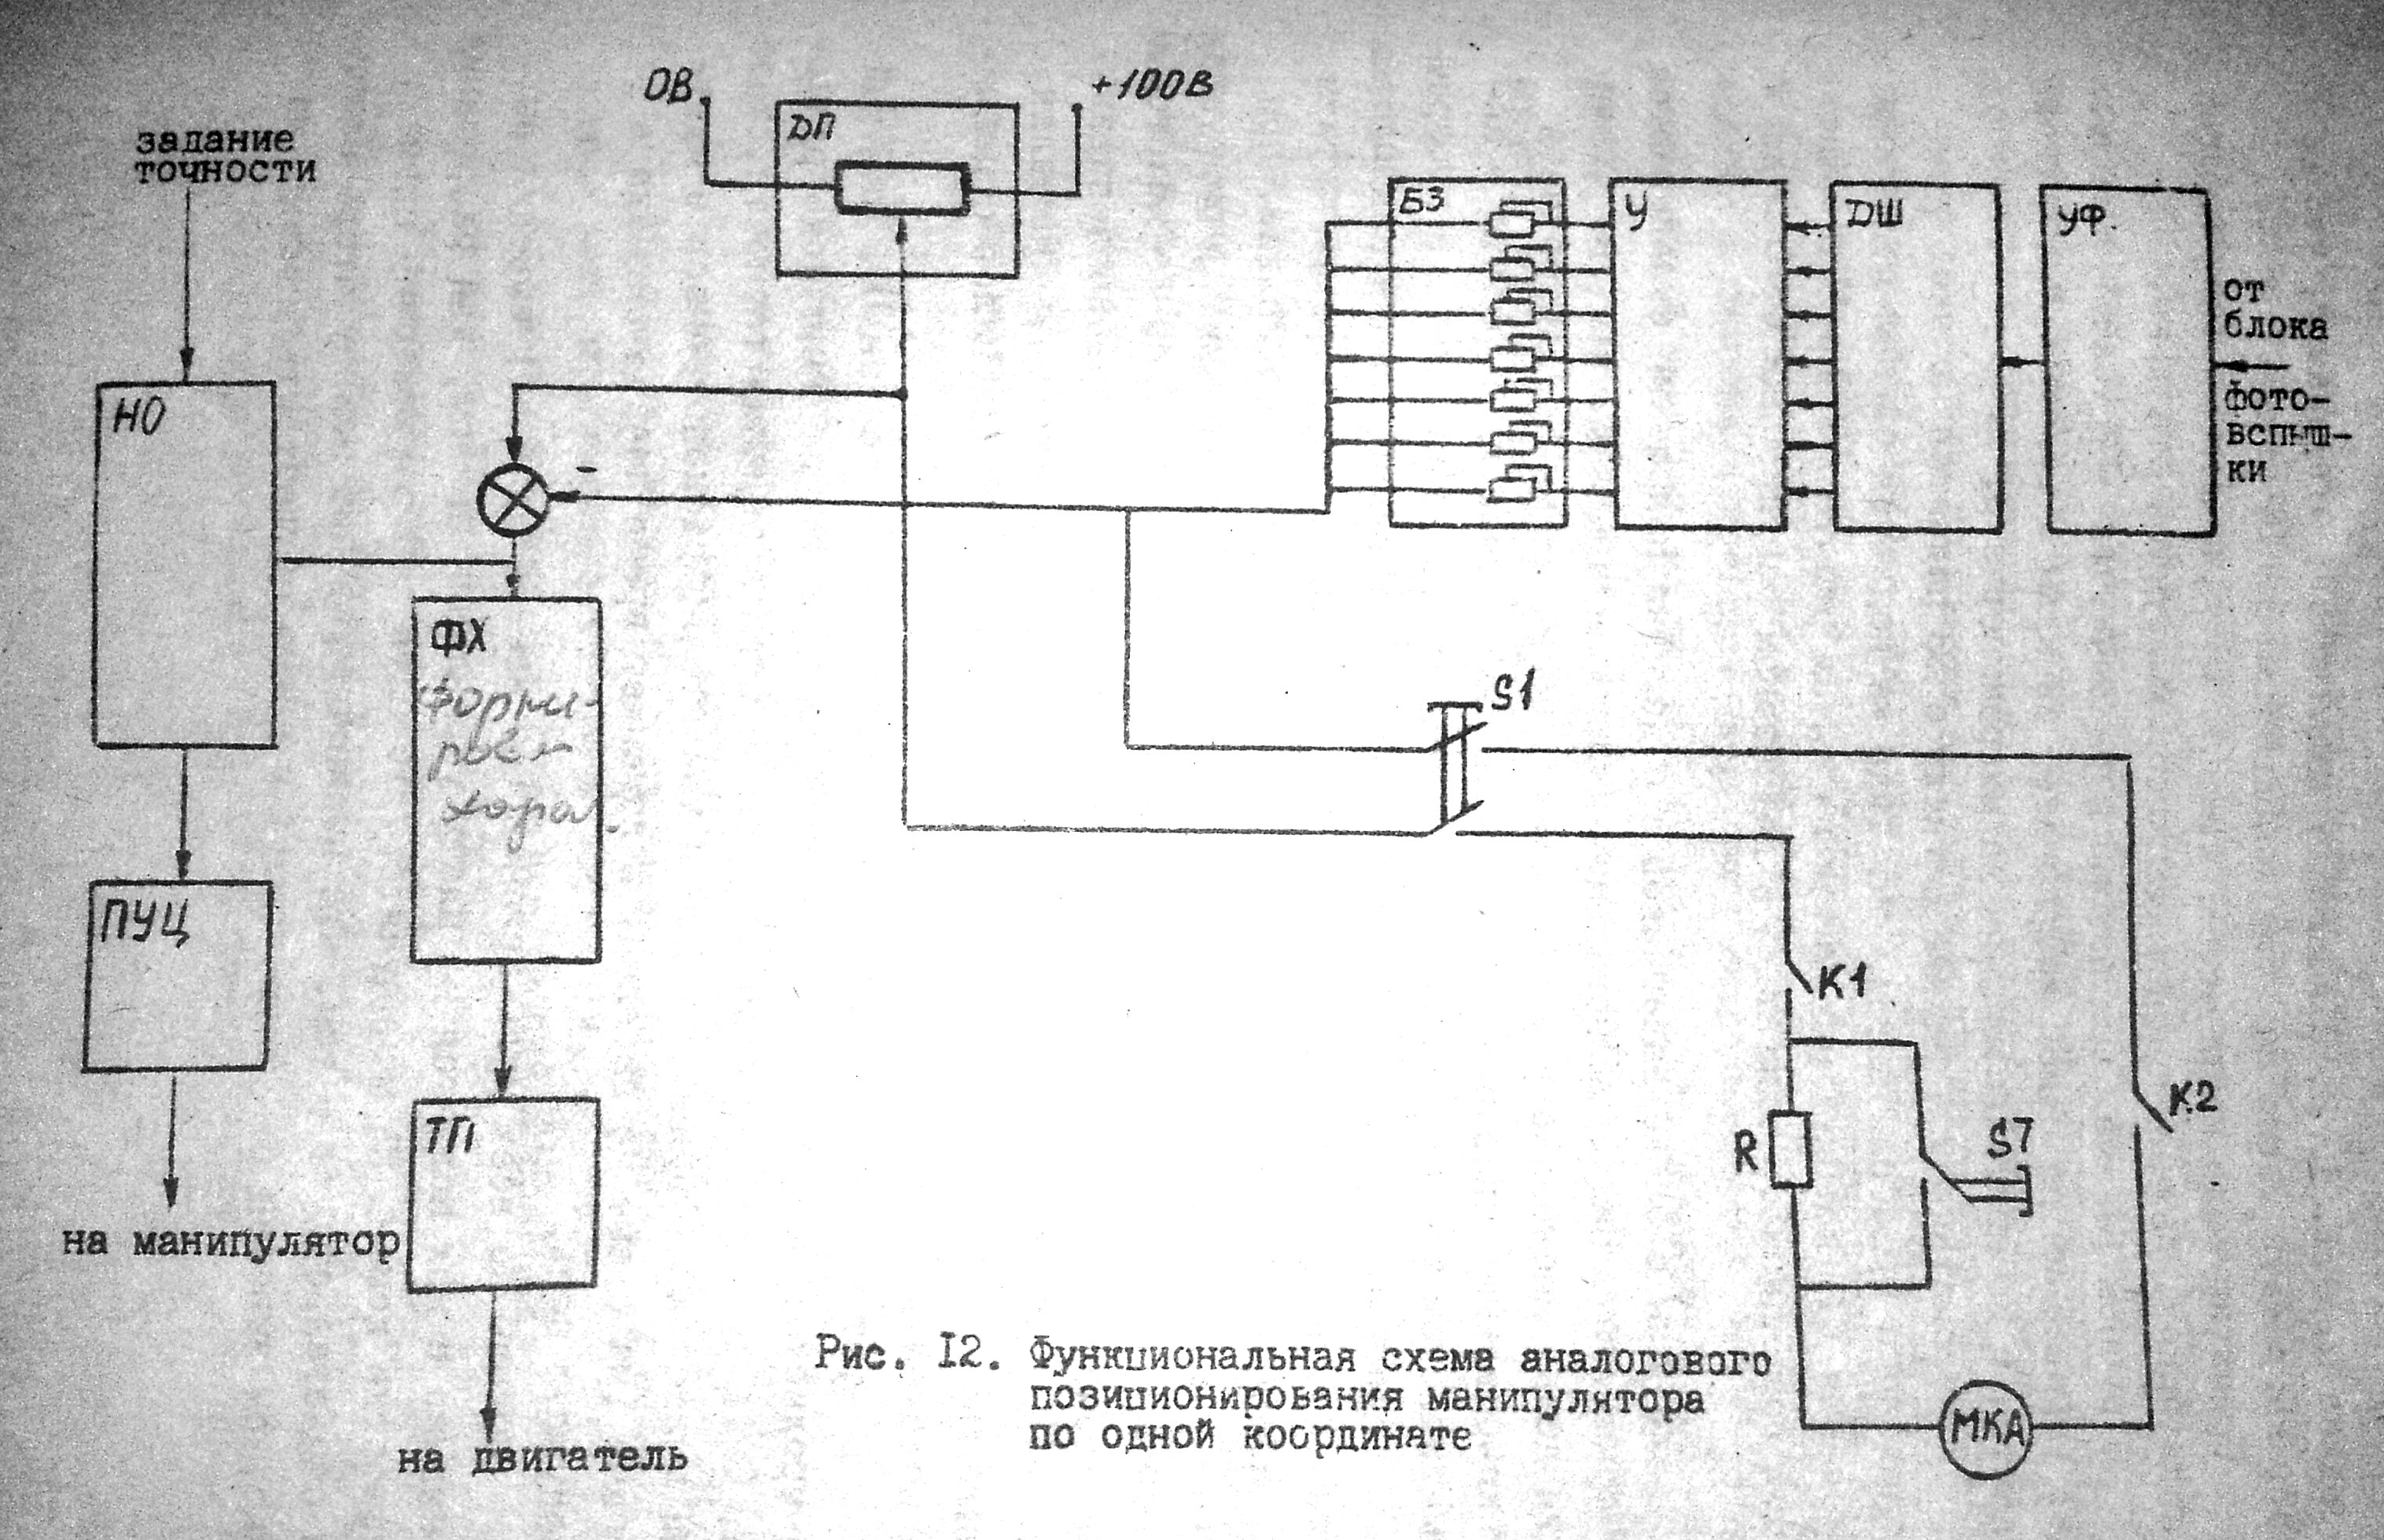
\includegraphics[width=1\linewidth]{Figures/functional.png}
    \caption{Функциональная схема аналогового позиционирования манипулятора по одной координате}
    \label{fig:functional}
\end{figure}

\subsection*{Исполнительные механизмы ПР ``Универсал 5.02''}

\begin{itemize}
    \item механизм поворота (электродвигатель, червячная и цилиндрическая передачи);
    \item механизм подъема (2 электродвигателя, передача винт-гайка, пантограф);
    \item механизм схвата (пневмоцилиндр, ползунно-рычажный механизм);
    \item сгибание схвата (пневмоцилиндр, реечно-зубчатая передача);
    \item вращение кисти (планетарная передача, ползун-водило, пневмоцилиндр);
    \item механизм радиального вращения руки (ЭД, цилиндрическая передача, зубчато-реечная передача);
    \item поворот руки (ЭД, цилиндрическая и червячная передачи).
\end{itemize}

\subsection*{Датчики транспортные}

\begin{itemize}
    \item потенциометры;
    \item АОС положения;
    \item АОС скорости;
    \item тахогенераторы;
\end{itemize}

\subsection*{Ориентирующие датчики}

\begin{itemize}
    \item жесткий упор;
    \item демпфирующее устройство.
\end{itemize}
